\section{Zielsetzung}
Ziel dieses Versuchs ist es die Temperaturabhängigkeit der dynamischen Viskosität von destilliertem Wasser, mittels Kugelfall-Viskosimeter, zu bestimmen.
\section{Theorie}
\label{sec:Theorie}
Auf einen Körper wirkt eine Reibungskraft, welche von der Berührungsfläche $A$ und der Geschwindigkeit abhängt, sofern sich dieser durch eine Flüssigkeit bewegt.
Die Flüssigkeit selbst wird durch eine Materialkonstante und die dynamische Viskosität $\eta$ beschrieben.
Diese kann unter Verwendung eines Kugelfall-Viskosimeter bestimmt werden.
Hierbei fällt eine Kugel mit Radius $r$ in einer Flüssigkeit, sodass keine Wirbel entstehen.
Die Strömung ist dann laminar.
Dann kann die Stokessche Reibung durch
\begin{equation}
  F_R = 6 \pi \eta \upsilon r
\end{equation}
angeben werden, wobei \upsilon die Fallgeschwindigkeit darstellt.
Neben der Reibungskraft wirken auf die Kugel die Schwerkraft $F_g$ und der Auftrieb $F_A$.
Auftrieb und Schwerkraft sind entgegengerichtet.
\subsection{Aufbau}
Um die Viskosität zu betimmen wird hier das Kugelfall-Viskosimeter nach Höppler verwendet.
Die Abbildung\ref{fig:aufbau} zeigt dieses.
\begin{figure}[H]
  \centering
  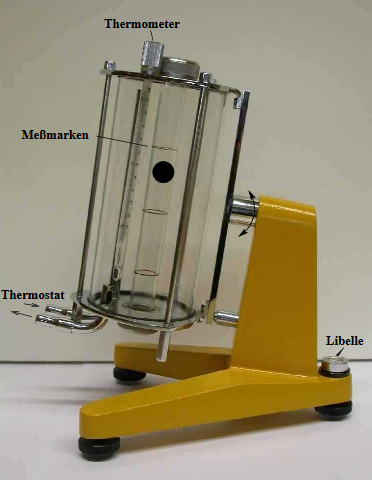
\includegraphics{content/Aufbau.png}
  \caption{Kugelfall-Viskosimeter nach Höppler\cite{v107}}
  \label{fig:aufbau}
\end{figure}
Bei diesem wird eine Kugel in einem Rohr fallengelassen, welches einen geringfügig größeren Durchmesser als die Kugel aufweist.
Das Rohr ist dabei mit einer viskosen Flüssigkeit gefüllt.
Um zu vermeiden, dass die Kugel unkontrolliert gegen die Rohrwand stößt ist das Fallrohr leicht geneigt, sodass die Kugel die Rohrwand hinabgleitet.
Bei konstanter Temperatur lässt sich die Viskosität der Flüssigkeit durch
\begin{equation}
  \upeta = K (\rho_K -\rho_\text{Fl}) \cdot t
\end{equation}
 berechnen.
Hier ist $\rho_K$ die Dichte der Kugel, $\rho_\text{Fl}$ die Dichte der Flüssigkeit und $K$ eine Apparaturkonstante, welch sowohl die Fallhöhe als auch die Kugelgeometrie enthällt.
Die Viskosität vieler Flüssigkeiten ist stark Temperaturabhängig.
Andradesches Gleichung beschreibt die Viskosität bei variabler Temperatur:
\begin{equation}
  \label{eq:and}
  \upeta (T)= A \exp(\frac{B}{T})
\end{equation}
A und B sind dabei Konstanten.
Die Temperatur der viskosen Flüssigkeit lässt sich über ein Wasserbad regulieren, welches durch eine Pumpe realiesirt wird.
Nachdem die Kugel am Ende des Fallrohrs angekommen ist kann das Viskosimeter um $180$ Grad rotiert werden.
\subsection{Die Reynoldsche Zahl}
Die Reynoldsche Zahl ist eine dimensionslose Kenngröße.
Sie findet Verwendung bei der Untersuchung ob eine Strömung turbulent oder laminar ist.
Überschreitet diese einen kirtischen Wert, so ist die Strömung turbulent.
Für Wasser liegt dieser Wert bei $R_e=2300$\cite{ström}.
Die Reynoldsche Zahl ist durch
\begin{equation}
  R_e = \frac{\rho \nu d}{\upeta}
\end{equation}
definiert.
Hierbei ist \rho die Dichte der Flüssigkeit, \nu die Strömungsgeschwindigkeit der Flüßigkeit gegenüber des Körpers und $d$ die Länge des Körpers.
